\documentclass[tikz,border=4pt]{standalone}
\usepackage{amsmath}
\begin{document}
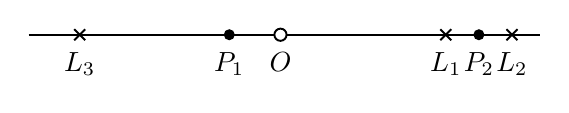
\begin{tikzpicture}[>=stealth, thick, scale=1.0]
  % x-axis line
  \draw[line width=0.6pt] (-3.2, 0) -- (3.3, 0);

  % Cross mark macro helper via path
  \def\cross#1{%
    \draw[line width=0.7pt] (#1-0.07, -0.07) -- (#1+0.07, 0.07);%
    \draw[line width=0.7pt] (#1-0.07, 0.07) -- (#1+0.07, -0.07);%
  }

  % L3, P1, O, L1, P2, L2
  \cross{-2.55}
  \node[below] at (-2.55, -0.10) {$L_3$};

  \fill (-0.65, 0) circle (2.0pt);
  \node[below] at (-0.65, -0.10) {$P_1$};

  \draw[fill=white, line width=0.7pt] (0, 0) circle (2.2pt);
  \node[below] at (0, -0.10) {$O$};

  \cross{2.10}
  \node[below] at (2.10, -0.10) {$L_1$};

  \fill (2.52, 0) circle (2.0pt);
  \node[below] at (2.52, -0.10) {$P_2$};

  \cross{2.94}
  \node[below] at (2.94, -0.10) {$L_2$};
\end{tikzpicture}
\end{document}
